\documentclass[10pt,a4paper]{article}
\usepackage[utf8]{inputenc}
\usepackage[english]{babel}
\usepackage[T1]{fontenc}
\usepackage{amsmath}
\usepackage{amsfonts}
\usepackage{amssymb}
\usepackage{makeidx}
\usepackage{graphicx}
\usepackage{fourier}
\usepackage{listings}
\usepackage{color}
\usepackage{hyperref}
\usepackage[left=2cm,right=2cm,top=2cm,bottom=2cm]{geometry}
\author{Johannes Scheller, Vincent Noculak, Lukas Powalla}
\title{Computational Physics - Project 1}
\begin{document}
\lstset{language=C++,
	keywordstyle=\bfseries\color{blue},
	commentstyle=\itshape\color{red},
	stringstyle=\color{green},
	identifierstyle=\bfseries,
	frame=single}
\maketitle
\newpage
\tableofcontents
\newpage
\section{Introduction to Project 1}
In physics, we often have to deal with differential equations o second order, which can be generally written in the from
\begin{equation}
	\frac{d^{2}y}{dx1{2}}+k^2(x)y=f(x)\quad,
\end{equation}
where we call $f$ the inhomgeneous term and $k^2(x)$ is a real function. A special case of these cases is Poisson's equation, which reads in the one-dimensional, spherical case
\begin{equation}
	\frac{1}{r^2}\frac{d}{dr}\left(r^2\frac{d\Phi}{dr}\right)=-4\pi\rho\left(\mathbf{r}\right)\quad.
\end{equation}
Doing some substitutions, we can write this in the following, more general form:
\begin{equation}
	\label{diff}
	-u''(x)=f(x)
\end{equation}
In this project, we try to solve eq.\eqref{diff} with the boundary conditions $u(0)=u(1)=0$. Therefore, we have to discretize $f$ and $u$. We approximate $u(x)$ as $v_i$, using a grid of $n$ gridpoints $x_i=i\cdot h$. Thus, $h=1/(n+1)$ is our steplength. We will also write $f_i=f(x_i)=f(hi)$.\\Approximating the second derivative of $u$, we get
\begin{equation}
	\label{num}
	-\frac{v_{i+1}+v_{i-1}-2v_i}{h^2}=f_i
\end{equation}
Our goal is to solve this equation \eqref{num}. Therefore, we will rewrite it as a set of linear equations in matrix form.

\subsection{Rewriting the equation in matrix-form}
Eq \eqref{num} can be written as a set of linear equations in matrix form. Therefore, we have to do the following steps:
\begin{align}
	-\frac{v_{i+1}+v_{i-1}-2v_i}{h^2}&=f_i\nonumber\\
	\label{vorform}-\left(v_{i+1}+v_{i-1}-2v_i\right)&=h^2\cdot f_i\\
\end{align}
Assuming we have an $n\times n$-matrix $\mathbf A$ of the following form

\begin{equation}
{\bf A} = \left(\begin{array}{cccccc}
2& -1& 0 &\dots   & \dots &0 \\
-1 & 2 & -1 &0 &\dots &\dots \\
0&-1 &2 & -1 & 0 & \dots \\\dots
& \dots   & \dots &\dots   &\dots & \dots \\
0&\dots   &\dots  &-1 &2& -1 \\
0&\dots    &\dots  & 0  &-1 & 2 \\
\end{array} \right)\quad,
\end{equation}
then we can rewrite this matrix in index notation as
\begin{equation}
\label{index}
	a_{ij}=\begin{cases}
		2&\mbox{if }i=j\\
		-1&\mbox{if  }|i-j|=1\\
		0&\mbox{else}
	\end{cases}\quad.
\end{equation}
Using this, we can also rewrite the multiplication $\mathbf{w}=\mathbf{A}\cdot\mathbf{v}$ with an $n$-dimensional vector $\mathbf v$ in the following way:
\begin{equation}
	w_i\quad\underset{\mathrm{def}}{=}\quad\sum_{j=1}^{n}a_{ij}\cdot v_j\quad\underset{\eqref{index}}{=}\quad -v_{i-1}+2v_i-v_{i+1}
\end{equation}
By using this result and substituting $h^2\cdot f_i\rightarrow\bar{b}$ in eq \eqref{vorform}, we get to the following equation:
\begin{equation}
	\mathbf{A \cdot v}=\bar{\mathbf{b}}
\end{equation}
with matrix $\mathbf{A}$ as given above. This is a set of linear equations that we are going to solve with our programm. In this example, we will assume that $f(x)$ is given by $f(x)=100\mathrm{e}^{-10x}$. Thus, the analytical solution of eq \eqref{diff} is given by $u(x)=1-(1-\mathrm{e}^{-10})x-\mathrm{e}^{-10x}$. We will later compare our numerical results to this solution.

\section{Different algorithm to solve this set of linear equations}

In this chapter, We want to solve the given set of linear equations first by solving it with a self-programmed algorhithm. Furthermore, we want to compare the produced numerical solution to the exact solution and calculate the maximum relative error for a given number of Gridpoints. 
In order to know, whether our algorithm is best to solve this set of linear equations, we want to compare this algorhith with LU-decomposition and Gaussian algorhitm with respect to the floating point operations and the calculation time. 

\subsection{self-programmed algorithm }

As we have shown in the previous capture, you can rewrite the set of linear equations as product of a matrix and a vector:
\begin{equation}
	\mathbf{A \cdot v}=\bar{\mathbf{b}}
\end{equation}
In this case, the matrix A is a tridiagonal matrix. This means, that it is possible to interpret this matrix as 3 vectors because all other components of the matrix are zero and will stay zero. This gives us the advantage that we don't have to deal with 2-dimensional Arrays and we can dump the number of floating operations (compared to LU-decomposition/Gaussian-algorithm)

The programmed algorithm will work in the following way. First, we want to reach a upper diagonal matrix by vector-additions/subtractions. Second, We want to bring the matrix to a diagonal form and at last, we scale the solution vector. The first two steps also effekt the solutionvector (in our case btilde[] ). We programmed following souce-code (extract):

extract of the used algorithm((12 floating operations):
\begin{lstlisting}
//first
for(int i=0;i<n;i++){
	b[i+1]=b[i+1]-c[i]*(a[i+1]/b[i]);
	btilde[i+1]= btilde[i+1]-btilde[i]*(a[i+1]/b[i]);
}
//second
for(int i=n-1;i>0;i--){
	btilde[i-1]=btilde[i-1]-btilde[i]*(c[i-1]/b[i]);
}
//normalization
for(int i=0;i<n;i++){
	btilde[i]=btilde[i]/b[i];
}
\end{lstlisting}
	
	
As you can see, we use at the moment 12n floating point operations for the mainalgorithm. If we look closer at the algorithm, we will see that you can simplify a lot by skipping unnecessary arithmetic operations. 
We managed to get to 7 Floating point operations:
\begin{lstlisting}
//first
for(int i=0;i<n;i++){
	b[i+1]=2-1/b[i];
	btilde[i+1]= btilde[i+1]+btilde[i]/b[i];
}
//second
for(int i=n-1;i>0;i--){
	btilde[i-1]=btilde[i-1]+btilde[i]/b[i];
}
//normalization
for(int i=0;i<n;i++){
	btilde[i]=btilde[i]/b[i];
}
\end{lstlisting}
	
\subsection{Gaussian elimination}

The standard algorithm to solve any system of linear equations of the form $\mathbf{A}\cdot\mathbf{x}=\mathbf{v}$ is the so called Gaussian elimination. It uses only elementary row operations on the matrix. First, we perform a forward substitution to transform $A$ into an upper triangular matrix. Than, a backward substitution transforms it into diagonal form.

For the forward substituion, we need $\frac{n^3+n^2}{2}$ FLOPs, and another $\frac{3n^2}{2}$ for the backward substituion. The normalization needs another n FLOPs, so we end up with a total of $\frac{n^3}{2}+2n^2+n$ FLOPs for solving our problem by using Gaussian elimination.(see extract of the algorithm)

\begin{lstlisting}
//Forward substitution
double factor;
for(int outerLine=0 ; outerLine<n ; outerLine++){
  for(int innerLine=outerLine+1; innerLine<n;innerLine++){
      //Column [o] of every line [o+i] should be 
      //equal to zero by adding (factor*Matrix[o][o])
      factor=-A[innerLine][outerLine]/A[outerLine][outerLine];
      for(int column=outerLine;column<n;column++){
          A[innerLine][column]+=factor*A[outerLine][column];
      }
      btilde[innerLine]+=factor*btilde[outerLine];
  }
}
//Backward substitution
for(int outerLine=n-1; outerLine>=0; outerLine--){
  for(int innerLine=outerLine-1; innerLine>=0; innerLine--){
     btilde[innerLine]-=btilde[outerLine]*(A[innerLine][outerLine]/A[outerLine][outerLine]);
  }
}
//Normalization
for(int i=0;i<n;i++){
    btilde[i]=(btilde[i]/A[i][i]);
}
\end{lstlisting}

\subsection{LU-decomposition}

In the LU-decompsition we factorize the matrix $\mathbf A$ as the product of a lower($\mathbf L$) and an upper($\mathbf{U}$) triangular matrix. As a consequence we get the following equation:

\begin{equation}
\mathbf{L \cdot U \cdot v = \bar{b}}
\end{equation}

If we say $\mathbf{U \cdot v = w}$, we get two systems of linear equations which need to be solved.

\begin{gather}
\mathbf{L \cdot w = \bar{b}} \\
\mathbf{U \cdot v = w}
\end{gather}

While solving (14) and (15) only need $\sigma(n^2)$ flops, which is less compared to the gaussian elimination, factorising $\mathbf{A}$ as in (12) takes $\sigma(n^3)$ flops. In total the LU-decomposition does take to the power of two flops more than our algorithm. (which means $\sigma(n^3)$ flops in total)


\section{Resuluts and discussion of the self-programmed algorithm}

We solved the linear set of equation with a different number of Gridpoints. This means, that we discretise the used funktions and approximated them with n Gridpoints. If you take a closer look at the given solutions produced with our algorithm, you will notice that the numerical approximation seems to converge to the exact solution. (for n=10...$10^5$) In the figure \ref{Comparison10}, you can see the numerical solution for 10 Gridpoints. The numerical approximation fits very well with the exact solution, however the boundary conditions seem to be fullfilled. We run our programm with diferend numer of Gridpoints. The figure with 100 Gridpoints you can find in figure \ref{Comparison100}, the figure with 1000 Gridpoints you can find in \ref{Comparison1000} and the figure with $10^5$ Gridpoints you can find in figure \ref{Comparison100000}. 



\begin{figure}[h]
\centering
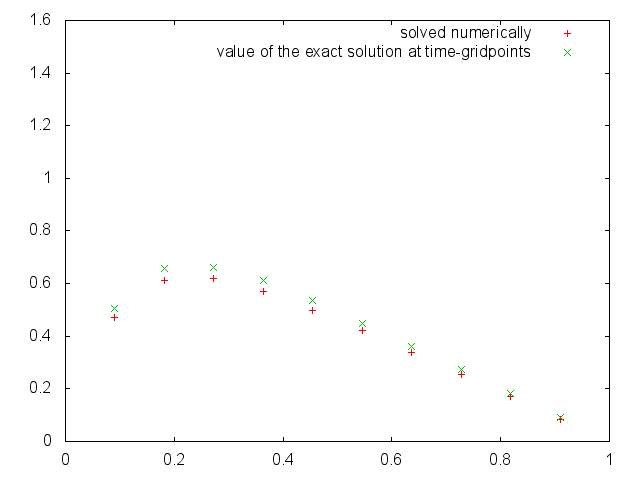
\includegraphics[scale=0.5]{Comparisonplot10.png}
\caption{Plot of the exact solution and the numerical solution for 10 Gridpoints}
\label{Comparison10}
\end{figure}

\begin{figure}[h]
\centering
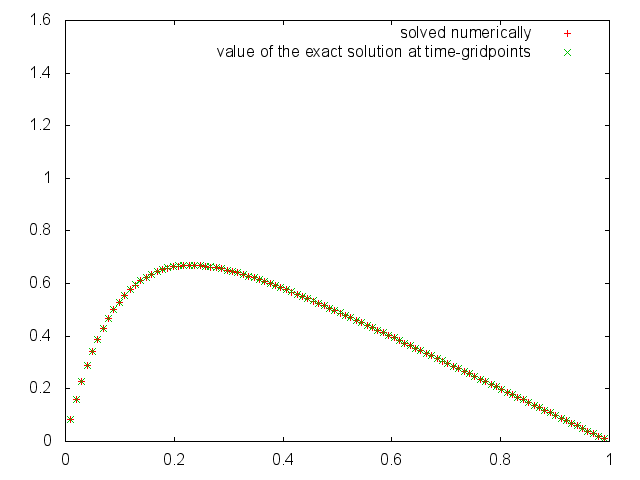
\includegraphics[scale=0.5]{Comparisonplot100.png}
\caption{Plot of the exact solution and the numerical solution for 100 Gridpoints}
\label{Comparison100}
\end{figure}

\begin{figure}[h]
\centering
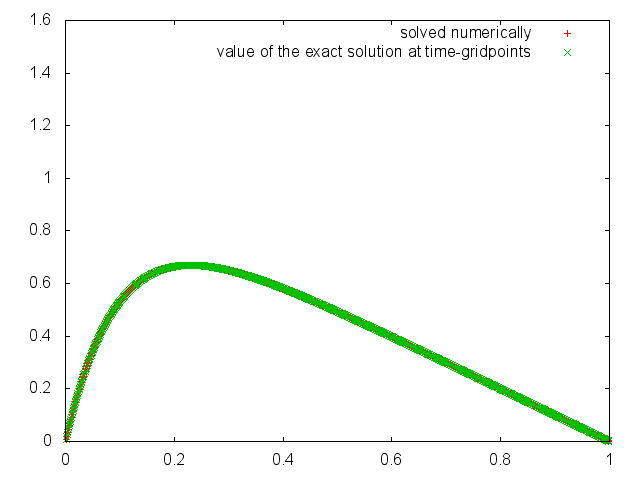
\includegraphics[scale=0.5]{Comparisonplot1000.png}
\caption{Plot of the exact solution and the numerical solution for 1000 Gridpoints}
\label{Comparison1000}
\end{figure}

\begin{figure}[h]
\centering
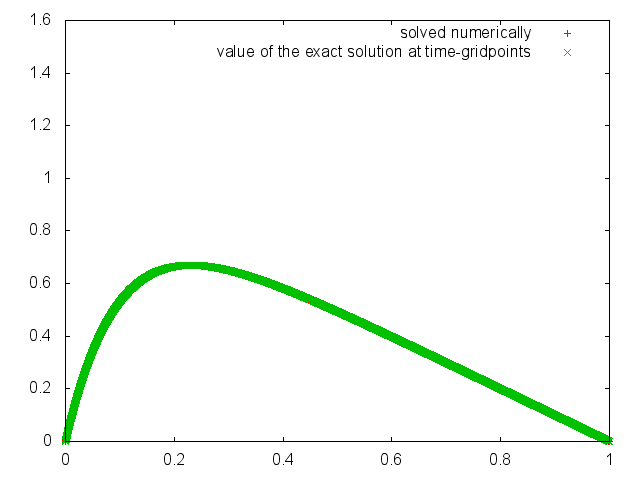
\includegraphics[scale=0.5]{Comparisonplot100000.png}
\caption{Plot of the exact solution and the numerical solution for 100000 Gridpoints}
\label{Comparison100000}
\end{figure}

In the next step, we want to compare our results with the exact solution. Therefore, we estimated the relative error for different step length. 
The relative errors can be computed with the expression \ref{equation rel error}. 

\begin{align}
R_{rel err.} = \left| \frac{v_i-u_i}{u_i} \right| \label{equation rel error}
\end{align}

We calculated the relative error for each number of Gridpoints as you can see in table \ref{max rel err}. The relative error decreases with an increasing number of Gridpoints. However, when you look at figure \ref{linear plot} you can see, that if you calculate the relative error for larger numbers of Gridpoints, the relative error will increase again.
In figure \ref{linear plot} we plottet following quantities:
\begin{align}
\mathrm{abscissa:} \quad &log_{10}\left(\frac{1}{1+n}\right) \\
\mathrm{ordinate:} \quad &log_{10} \left(\left| \frac{v_i-u_i}{u_i} \right| \right)
\end{align}
The minimum of the relative error  for approximately $n=10^{12}$. This can be explained by the effekt of loss of precision. 


\begin{table}
\centering
\caption{maximum relative error}
\label{max rel err}
\begin{tabular}{c|c|c}
n & h & maximum relative error\\
\hline\hline
10 & 0.0909091 & 0.0661153\\
100 & 0.00990099 & 0.000816513\\
1000 & 0.000999001 & 8.31665e-006\\
10000 & 9.999e-005 & 8.33134e-008\\
100000 & 9.9999e-006 & 1.43557e-009\\
\end{tabular}
\end{table}

\begin{figure}[h]
\centering
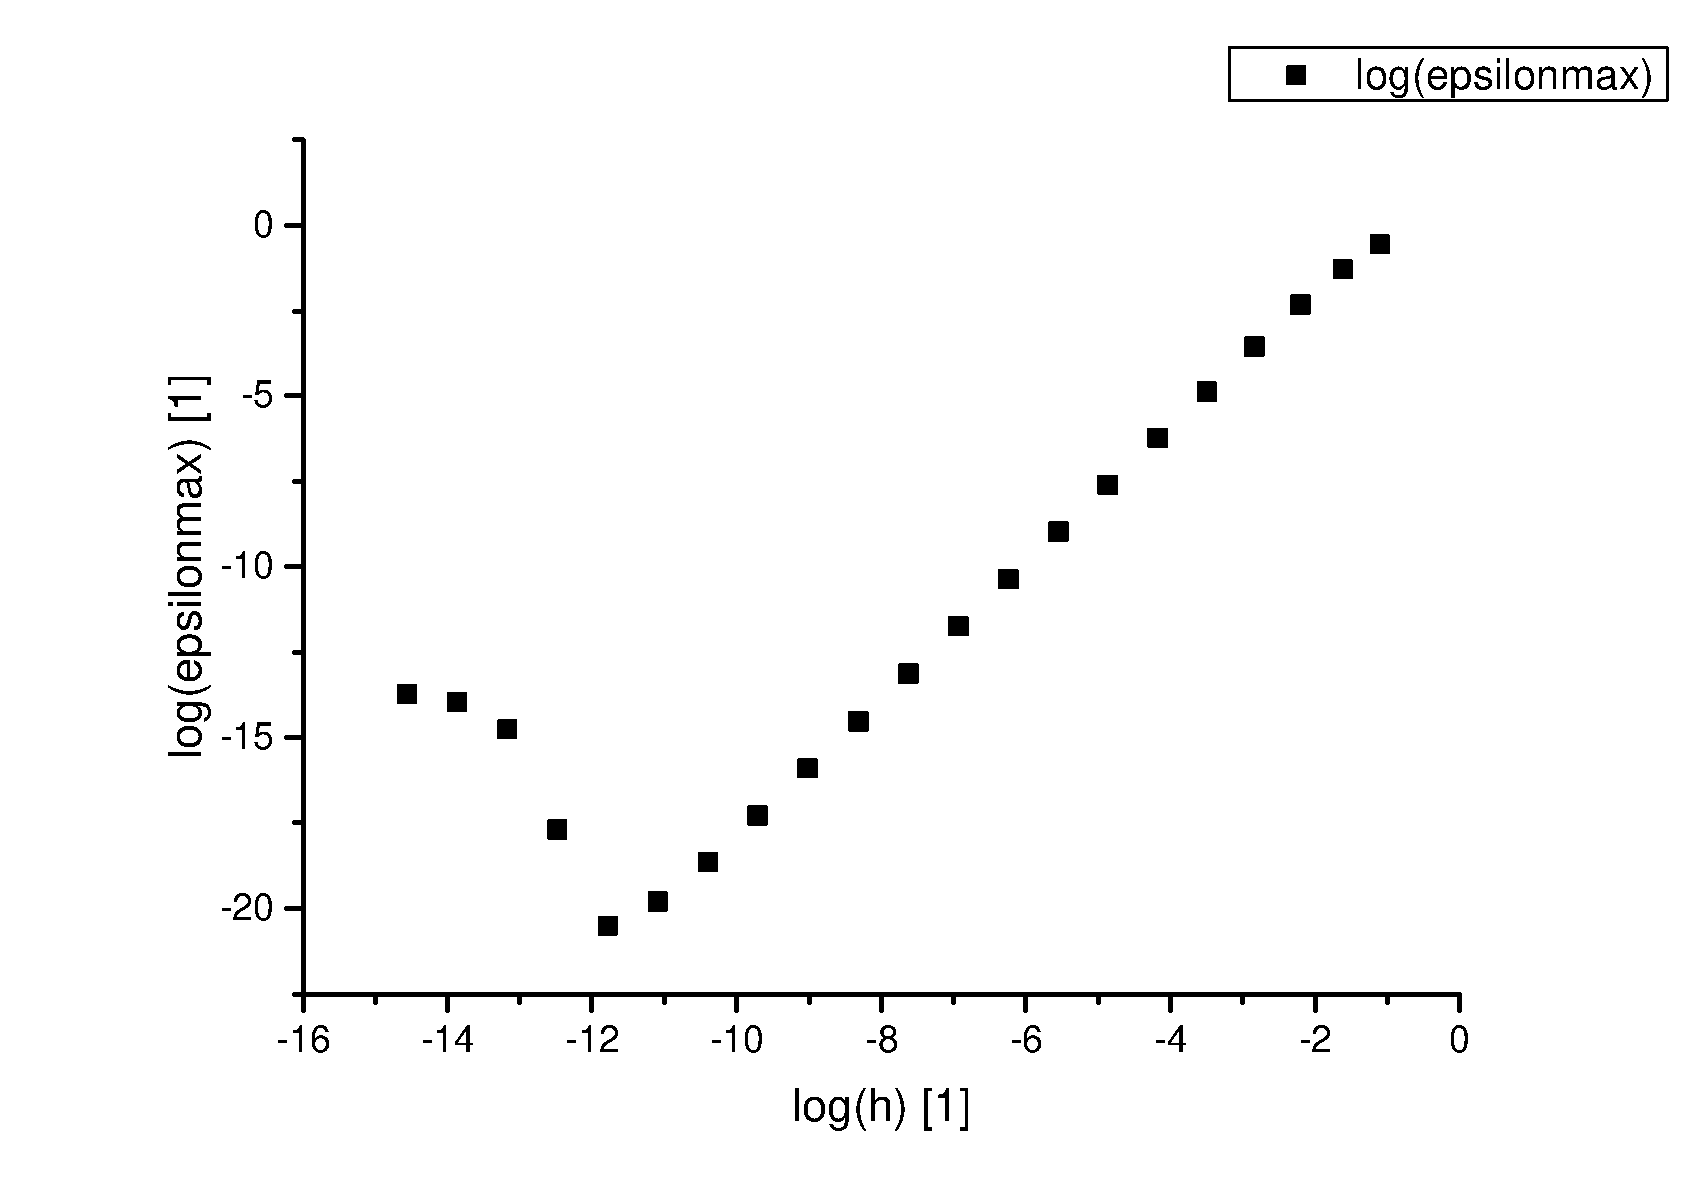
\includegraphics[scale=0.5]{epsilon_plot_log.pdf}
\caption{The epsilon is the maximum of the Epsilonerror for given Number of Gridpoints n (and Steplenght h) }
\label{linear plot}
\end{figure}

\section{Comparison of self-programmed algorithm, Gaussian elemination and LU-Decomposition }

We implemented our own Gaussian elimination algorithm in a program and we used the armadillo library (and blas/lapack) to solve the set of linear equations with LU-Decomposition. The results for a given number of Gridpoints were exactly the same. 

We can clearly see in tab \ref{LU tridiagonal time} for large values of $n$ that our tridiagonal solver is a lot faster than the one using LU-decompostion. This is due to the fact that the number of FLOPs for LU-decomposition is proportional to $n^3$, whereas the number of FLOPs for our tridiagonal solver is $7n$. We are not sure why the LU-decomposition is faster for small  $n$.
We cannot run LU-Decomposition with $n=10^{5}$. For this number of Gridpoints the matrix has $10^10$ elemants, whitch takes $8 \cdot 10^10$ bytes of memory because we initialized the matrixelements as double. This is equal to 80 GB. This is a many times higher than the ram of our computer. Therefore, we can't run the program like this. 

To draw a conclusion we have to say, that the different algorithm are useful for different problems. The gaussian elimination algorithm solves sets of linear equation in general. (with arbitrary matrix A) 
The LU decomposition might be useful if you want to solve the problem for different fuktions f(x), but with the same matrix A. LU decomposition is also very useful when you want to calculate the inverse of a matrix. The tridiagonal solver fits best for the given problemset. It needs the smallest numbers of FLOPS. 

\begin{table}
\centering
\caption{time measurement LU-decomposition}
\label{LU tridiagonal time}
\begin{tabular}{c|c|c}
n & LU-decomposition t/s & tridiagonal solver t/s \\
\hline\hline
10  &0 & 0.023\\
100  &0.002 & 0.007\\
1000 & 0.132 & 0.054\\
5000 & 4.448 & 0.248\\
\end{tabular}
\end{table}


\section{Source-code}

The source-code to all our programs can be found under the following link:

\url{https://github.com/Lupo191/Project1_Noculak_Scheller_Powalla/}

\end{document}